%! Author = Saeid Yazdani
%! Date = 9/7/2024


\section{Source-Follower Measurements}
\label{source-follower-measurements}

As stated before, the source follower multiplies the current
capabilities of the power amplifier according to the transconductance of the
used \acs{MOSFET}s on the high and low sides.
A series of measurements were carried out on the source-follower to
find design issues and perform optimization.

The bias currents of the LEDs are measured to be around \SI{1}{\milli\ampere} and
a voltage drop of \SI{1.6}{\volt} at high differential resistance.

The high-side \acs{MOSFET} (IXFH14N80P) shows an input capacitance of
\SI{3.9}{\nano\farad} and for the low-side \acs{MOSFET} (IXFH16P60P)
\SI{5.2}{\nano\farad}.

The small difference of the gate capacitances of the high-side and
low-side \acs{MOSFET}s leads to an imbalance in
turn-on and turn-off timings, since the gate capacitance determines how
quickly the \acs{MOSFET}s turn on or off.

The gate capacitance mismatch affects the load handling conditions as the slower
\acs{MOSFET} leads to less efficient energy transfer or higher stress on
the other \acs{MOSFET}.

Therefore, the gate drivers for both \acs{MOSFET}s must be adjusted in a way
that the difference in switching times is minimized.
This can be achieved by altering the current and/or voltage used for driving
each \acs{MOSFET}.


\begin{figure}[h!]
    \centering
    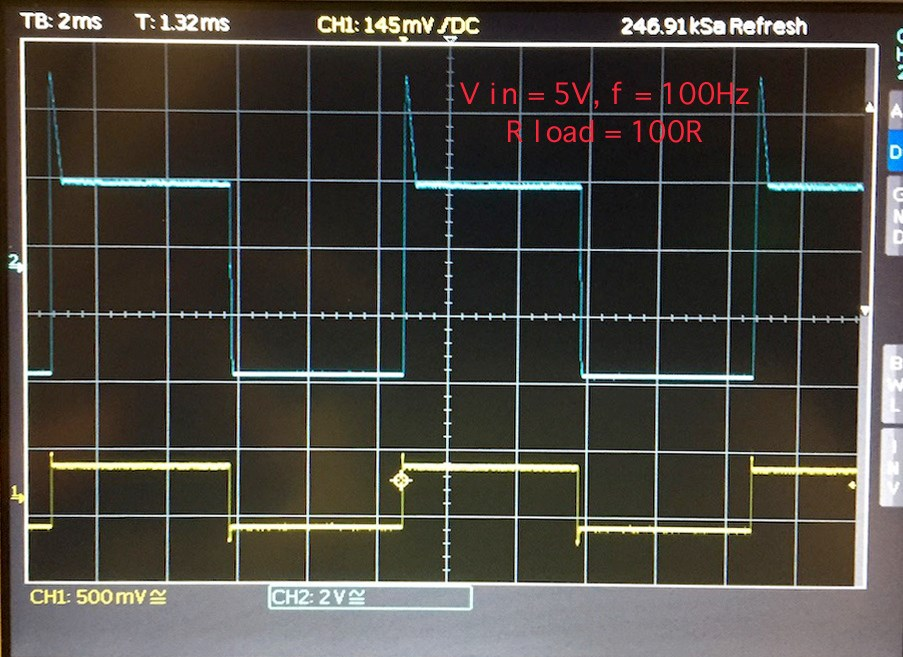
\includegraphics[scale=0.32]
    {figures/tests/amptest/sf_static}
    \caption[Power Stage Static Behavior]{
        Static behaviour of the power stage for a \SI{100}{\hertz}
        signal.
        $V_{IN}$ = \SI{5}{\volt} and $R_{LOAD}$ = \SI{100}{\ohm}
        \textbf{Blue Signal:} Source-Follower output.
        \textbf{Yellow Signal:} Pre Amplifier output.
        \SI{2}{\milli\second} Timebase.
    }
    \label{fig:power-stage-static-behacior}
\end{figure}


\begin{figure}[ht]
    \centering
    \begin{minipage}{0.48\textwidth}
        \centering
        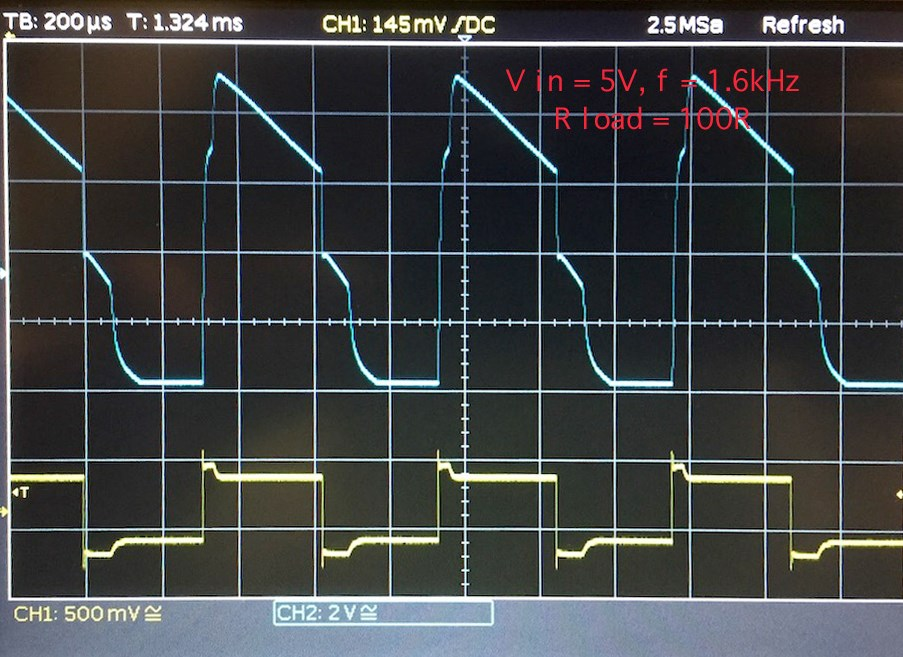
\includegraphics[width=\textwidth]{figures/tests/amptest/sf_dynamic-1dot6khz}
        \subcaption{$V_{IN}$ = \SI{5}{\volt}, $Freq.$ = \SI{1.6}{\kilo\hertz} and $R_{LOAD}$ = \SI{100}{\ohm}}
    \end{minipage}
    \hfill
    \begin{minipage}{0.48\textwidth}
        \centering
        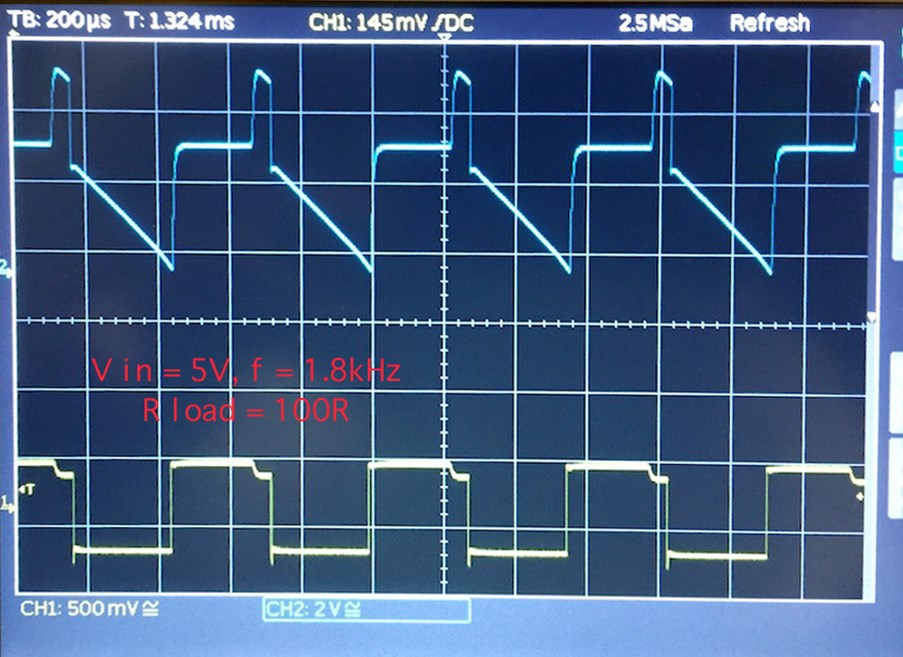
\includegraphics[width=\textwidth]{figures/tests/amptest/sf_dynamic-1dot8khz}
        \subcaption{$V_{IN}$ = \SI{5}{\volt}, $Freq.$ = \SI{1.8}{\kilo\hertz} and $R_{LOAD}$ = \SI{100}{\ohm}}
    \end{minipage}
    \caption[Power Stage Dynamic Behavior]{
        Dynamic behavior of the power stage. Stop frequency is \SI{1.8}{\kilo\hertz}.
        \textbf{Blue Signal:} Source-Follower output.
        \textbf{Yellow Signal:} Pre Amplifier output.
        \SI{200}{\micro\second} Timebase.
    }
    \label{fig:power-stage-dynamic-behacior}
\end{figure}
